%!TEX options = --shell-escape


\documentclass[doctor]{thesis-uestc}
\usepackage{xeCJK}
\usepackage{CJKutf8}

\usepackage{lscape}

\usepackage{amsmath}
\usepackage{algorithm}
\usepackage[noend]{algpseudocode}
\usepackage{xcolor}
\usepackage{makecell}
\usepackage{multicol}

\title{Research on Deep Learning} %论文标题
%\title{Research on Multi-Resolution Wavelet Deep Neural Network and Its Applications} %论文标题

\titleEn{Research on Deep learning} %英文标题
%\titleEn{Research on Multi-Resolution Wavelet Deep Neural Network and Its Applications} %英文标题

\author{Flora White Edson} 
%\author{Monday Happy Nkanta}
                                                     %作者

\authorEn{Flora White Edson}                                        
                                               %作者英文名
%\authorEn{Monday Happy Nkanta}                                               

\advisor{Professor James Lee}                                  %导师
\advisorEn{Professor James Lee}

%\advisor{Professor Jian Ping Li}                                  %导师
%\advisorEn{Professor Jian Ping Li}



%导师师英文名

\school{School of Computer Science and Engineering}                                        %学院英文名
\major{Computer Science and Technology}                                            %专业
\majorEn{Computer Science and Technology}           %专业英文名
\studentid{201814080018}

\begin{document}
\makecover  %封面

% abstract
\documentclass{standalone}
% preamble: usepackage, etc.
\begin{document}
	
\begin{chineseabstract}
英语语法纠错算法是指使用计算机编程技术自动识别和纠正非母语学习者所写中的英语文本中包含的语法错误。自动更正系统是 机器 学习的核心,可以应用于从英文文本数据中提取信息并构建可靠的语法校正方法。如何收集数据的方法是通过诊断和预测分析。使用的软件是自动更正的系统。

本文的目的是研究语法错误检查和纠正它们的系统。审查了四项研究概要,即文献综述,方法,实验和结果,以及结果,分析和讨论,并在两个数据集上进行指示和测试。一个数据集是自动更正的系统评论,将拼写错误的单词更改为正确的拼写。另一个数据集命令函数,其执行代码以提供输出。本文的研究结果为基于自动转换系统的进一步研究英语语法纠错提供了一定的参考。



\chinesekeyword{自然语言处理,机器翻译,自动更正系统,语法错误识别和初学者和非原生英语扬声器.}
\end{chineseabstract}

\end{document} %中文摘要

\documentclass{standalone}
% preamble: usepackage, etc.
\begin{document}

\begin{englishabstract}
English grammar error correction algorithm refers to the use of computer programming technology to automatically recognize and correct the grammar errors contained in English text written by non-native language learners. Autocorrect system is the core of machnine learning, which can be applied to extracting information from English text data and constructing a reliable grammar correction method. The methodology on how data was collected is by diagnostic and predictive analysis. The software used is autocorrect system.

 The aim of this thesis is to study about the systematics of the grammatical error checking and correcting them. Four outline of the study are reviewed namely literature review, Methodology, Experiments & Results, and Results, Analysis & Discussion, and they are instructed and tested on two data sets. One data set is auto-correct system reviews, which changes a misspelled word into the correct spelling. Another data set commanding functions, which is executing the code to give an output. The study results of this paper provide a certain reference for the further research English grammar error correction based on autocorrect system.

    
\englishkeyword{Natural language processing, Machine translation, Autocorrect system, Grammar error identification, and Beginner and non-native English speakers.}
\end{englishabstract}

\end{document}
 %英文摘要

% table of contents
\thesistableofcontents   %目录

% list of figures
\thesisfigurelist

% list of tables
\thesistablelist

\clearpage
\pagenumbering{arabic}
\standardhead

% thesis contents
% the contents of this dissertation are organized in a folder called chapter.
% Each chapter is put in a separate .tex file label as c2.tex, c3.tex, ... and so on
% exordium is chapter 1

\documentclass{standalone}
% preamble: usepackage, etc.
\begin{document}

\thesischapterexordium

\textbf{\section{Overview and Background}}
Various machine vision applications, such as image recognition, identification and detection [1]–[10], use convolution neural networks as the main strategy. CNNs are increasingly being learnt on huge datasets and are being accelerated by increasingly better GPU machines, resulting in most advanced level performance as compared to conventional approaches. The popularity of CNN in machine vision can be attributed to two factors. To begin with, existing CNN-led solutions dominate various simple tasks, such as image super-resolution (SISR) [1], [2], [11], denoising [5], deblurring [12], compression[13], and reconstruction [6], by outperforming other approaches by a wide margin. Secondly, CNNs are also used as an extensiblecomponent that can be incorporated into traditional approaches, allowing them to be used more widely [12], [14], [15]. 

In machine vision, CNNs can be thought of as a non-linear projection from the source images to the output. Conventionally, bigger receptive field aids in increasing CNN's fitting capabilities and promotes effective performance by considering greater spatial details. Increasing the depth of the network, widening the filter size, or performing pooling procedure can all help to expand the receptive field. However, increasing the depth of the network or the filter size will unavoidably increase the cost of computing resource.  pooling procedure can increase the receptive field and ensure continuous improvement by decreasing the spatial dimension of the feature vector. Nonetheless, it is possible that details will be lost. By introducing "zero holes" in convolutional filtering through the method of dilated filtering suggested by the authors in [8] as a trade-off between the size of the receptive and accuracy. 

Notwithstanding, for a fixed value higher than one for the receptive field of the dilating filtering only considers sparse samples from the image input with square patterns, which can result in grid effect [16]. More so, caution should be exercise while widening the receptive field in order to prevent both increasing the cost of computing resource and perhaps sacrificing the performance. To overcome the aforementioned issues, we designed and implemented CNN-based techniques that aim to strike a balance between efficiency and performance. Particularly, we presented presented multi-resolution analysis of discrete wavelet transform convolution neural network which provides feature representations in different scales and frequencies for the first aspect and replaces pooling operations with discrete wavelet transform (DWT) for the second aspect. The multi-resolution feature representations holds majority of the image features while discarding inconsistent details that could affect the performance of the model whereas the suggested sub-sampling approach does not lose any image detail or transitional features owing to the dynamic capabilities of DWT. 

Furthermore, DWT captures both the position and frequency details of the feature vectors as a strategy to maintain texture details of multi-frequency feature representation [21], [22]. Additionally,  channel-wise concatenation strategy is utilized to merge feature vectors in order to enrich feature representation. We demonstrate that dilated filtering may be viewed as a particular variation of multi-resolution discrete wavelet transform CNN, and that the suggested approach is more generic and successful in widening the receptive field than previous approaches. This research attains satisfactory results that outperforms well-known models in image classification and identification task. In terms of sub-sampling procedure with DWT, this research work obtains better performance for images classification and identification compared to pooling layers. The model suggested in this study may have a substantially bigger receptive field yet attains satisfactory performance.


In this light, machine vision and image classification research has transitioned to deep learning approaches, which are regarded to be more dependable than classic machine learning techniques in terms of improving image recognition performance. \citeup{4}. The configuration of the human brain is made up of many units of neurons, which is the basis for which deep neural network is modeled after. Information is transmitted across layers that function similarly to the human brain, with neurons serving as unit processes. A variety of deep learning approaches are used in image classification applications, such as those developed by Grace et al. \citeup {6 – 9}. Convolution neural networks are utilized in medicine to extract characteristics from images, while in industries, CNN is utilized to extract behavioral patterns and attributes from signals and network data which are essential to this dissertation because deep learning frameworks provide effective and reliable assessment results.


In this dissertation, we utilize  multi-resolution analysis and discrete wavelet transform  approaches coupled with deep learning frameworks to effectively process and extract audio and image data in order to obtain an effective classification and identification.  performance. We presented several comparison with stand-alone deep learning models and state-of-the-art methods.

\textbf{\section{Problem Statement}}

Recent technological development and increasing digital transmission of information have resulted in the creation of massive amounts of information. These information are nearly by definition multimedia of all formats which includes video, images, audio and so on. For most internet consumers, image and audio messages are the major format of correspondence, especially with the introduction of smart devices. The massive rise in internet speed and storage space has only intensified this trend. Image data has been developed, communicated, and propagated rapidly recently, contributing significantly to the world's big data quantity.

The main purpose of this dissertation is to develop and implement highly effective wavelet multi-resolution deep learning framework that feed on both audio and image data capable of accomplishing good classification and identification performance despite the difficult behavior of examining audio and image  data with numerous attributes such as low quality, resolution variation, dimensionality, and different sampling rates and frequencies, which makes audio and image data comprehension very difficult. Despite the fact that advances in deep learning complexity and implementation have generated convincing and innovative success in image analysis and interpretation, there is still a major gap in audio analysis when compared to the more accurate image feature presentation. In most audio analysis, deep learning framework process the data in one-dimensional input sample format. Also,  though image analysis has been well explored, less research has been carried out in generating texture details from  audio data  for efficient  analysis.

\textbf{\section{Contribution and Significance}}

In conclusion, this dissertation examines the model construction and implementation of a multi-resolution discrete wavelet transform deep learning framework for obtaining good performance in image classification and identification. The data pre-processing aspect of this dissertation involves converting one-dimensional audio data into two-dimensional domain for effective training. There are four core model contribution is one of three major model contributions in this research; the first model is the multi-resolution analysis CNN framework. The second technique is the  multi-resolution analysis capsule network. The third approach is the super-resolution CNN framework, and the fourth model is the GAN-based super-resolution approach. The models are as follows:

\begin{enumerate}
    \item The capability of multi-resolution analysis for image classification and identification. This model incorporated multi-resolution analysis scheme into convolution neural network to achieve optimal performance compared to up-to-date stand-alone CNN techniques. The efficacy of the model construction is validated using  the following evaluation metrics; specificity,  ROC,  accuracy, and sensitivity on CICDDoS2019\citeup{10}, RSNA Pneumonia\citeup{26},  COVID-CXR\citeup{24}, CT-repository \citeup{25}, and NIH\citeup{23} dataset.
    
    
    \item An improved wavelet capsule network for accurately classifying images. This model is demonstrated by integrating wavelet into capsule network in a shared weighted fashion with continuous wavelet transform as a pre-processing technique to handle data dimensionality conversion. The efficacy of the model construction is validated using  the following evaluation metrics; specificity,  ROC,  accuracy, and sensitivity on MIT-BIH Normal Sinus Rhythm \citeup{21}, RSNA Pneumonia\citeup{26}, COVID-CXR\citeup{24}, CT-repository \citeup{25}, and NIH\citeup{23} dataset.
    
    
    \item  An efficient wavelet multi-resolution neural network with super-resolution CNN on chest x-ray (CXR) images for COVID-19 pneumonia identification. The Super-Resolution CNN (SRCNN) is used to effectively regenerate high-resolution (HR) CXR images from low-resolution (LR) CXR counterparts, addressing the issue of low CXR image resolution. The HR CXR images are then forwarded into the wavelet multi-resolution neural network, which extracts distinguishing characteristics for COVID-19 identification. The performance of the model is validated using well-known evaluation metrics as follows; accuracy, sensitivity specificity and ROC on RSNA Pneumonia\citeup{26}, COVID-CXR\citeup{24}, CT-repository \citeup{25}, and NIH\citeup{23} dataset.
    
    
    \item For fault diagnosis and classification, a super-resolution generative adversarial learning scheme is implemented. This scheme pits two neural networks, the generator and discriminator against one other to create new and artificial data instances that are regarded genuine. To produce deblurred and denoised HR images, the GAN-based system utilizes a connected nonlinear mapping derived from noise-polluted low-resolution input images. Accuracy, sensitivity, specificity, and ROC are the evaluation metrics adopted in this study using Case Western Reserve University dataset \citeup{38}.
    
    
\end{enumerate}

\textbf{\section{Organization and Outline of the Dissertation}}

The remaining chapters of this dissertation are structured as follows:

\begin{enumerate}
    \item \textit{Chapter 2}: This chapter provides a useful overview of the existing literature in wavelet transform, multi-resolution Analysis, and deep neural network. The existing strategies are addressed, along with their benefits, drawbacks, and suggestions for improvements.

    \item \textit{Chapter 3}: This chapter introduces the capability of multi-resolution analysis for image classification and identification. The model design incorporated wavelet multi-resolution analysis into Convolution Neural Networks for  the feature extraction and classification of images. The model's building blocks, design, and implementation, as well as enrich experimental analysis, are all thoroughly described.

    \item \textit{Chapter 4}: This chapter describes an improved wavelet capsule network for accurately classifying images. This approach is illustrated by incorporating wavelet into a shared weighted capsule network with continuous wavelet transform as a pre-processing module for converting one-dimensional time-domain audio signal into two-dimensional time-frequency domain scalogram. The scalogram becomes the input data to the wavelet capsule network for feature extraction and classification. 
    

    \item \textit{Chapter 5}: This chapter describes an effective wavelet multi-resolution neural network with super-resolution CNN for COVID-19 pneumonia diagnosis on chest x-ray (CXR) images. To address the issue of poor CXR image quality, the Super-Resolution CNN (SRCNN) is utilized to successfully regenerate high-resolution (HR) CXR images from low-resolution (LR) CXR counterparts. The wavelet multi-resolution neural network is then used to extract distinguishing characteristics for COVID-19 identification from the HR CXR images.
   
   
    \item \textit{Chapter 6}:  This chapter describes our modified super-resolution generative adversarial learning technique implemented for fault diagnosis and classification. This scheme pits two neural networks, the generator and the discriminator, against one another in order to generate new and artificial data instances that are considered genuine. The GAN-based system uses a connected nonlinear mapping obtained from noise-corrupted low-resolution input images to generate de-blurred and de-noised HR images.
    

    \item \textit{Chapter 7}: This chapter summarizes  and outlines the reported methodology and fundamental ideas of the dissertation, as well as proposing potential future study areas in the field of wavelet multi-resolution deep neural network for image analysis
    

\end{enumerate}


\end{document}  % Chapter 1 contents inside the chapter folder
\documentclass{standalone}
% preamble: usepackage, etc.
\begin{document}


\chapter{Literature Review}
\label{Chapter2}

In the field of vision understanding, Spatial and spectral approaches are two major approaches for image processing tasks such as image classification and object recognition. The tasks entail analyzing details in images using machine vision strategies and combining them with wavelet transforms analysis algorithms. This chapter examines the concept of wavelet analysis, convolution neural network, existing methods, their contributions, and their usefulness, and revealing a potential study area for the application of wavelet convolution neural network analysis.

\textbf{\section{Wavelet Transform Analysis}}
Time–frequency domain signal evaluation approaches allow for simultaneous explanation of the signal in terms of time and frequency , which permits better explanation of the local, temporary, or infrequent components. Many of the concepts that govern wavelet transforms have been around for decades. Nevertheless, as we know it today, wavelet transform analysis was first designed to investigate seismic data in the mid-1980s (Goupillaud et al 1984). During the rest of the 1980s, wavelet analysis continued to thrive within a small research domain, mostly mathematical society, with only a few scientific articles published every year. In the early 1990s, science and engineering got some breakthrough from the application of  wavelet transform, with a significant increase in the number of scholars focusing on wavelet transform during that period. Over 1500 peer-reviewed journal publications on the subject of wavelet transform application have been published in previous years, spanning a wide range of disciplines. Wavelet transforms today are divided into two types: continuous wavelet transforms and discrete wavelet transforms. These types will be looked at separately.

\textbf{\subsection{Continuous Wavelet Transform}}
Continuous wavelet transform (CWT) is an approach for analyzing  time–frequency which is different from the conventional short time Fourier transform (STFT) that allows for arbitrarily high frequency signal attribute localization in time. The CWT achieves this by using a changeable window width that is proportional to the observation scale. This adaptability allows for the seclusion of high frequency information. The CWT differs from the STFT in a way that it is not restricted to the use of oscillatory assessing functions, instead, a wide range of localized waveforms could be used depending if they meet certain mathematical conditions.






\end{document}        % Chapter 2 contents inside the chapter folder
\documentclass{standalone}
% preamble: usepackage, etc.

\begin{document}
\chapter{The Capability of Convolution Neural Network}
\label{Chapter3}

For diverse applications, several deep learning algorithms have been thoroughly examined, allowing for pattern and attribute understanding for the interpretation of both basic and complex representations. In the field of machine vision and learning, substantial advancements have recently been made. The convolution Neural Network (CNN) has advanced into a strong tool for perceptual image processing and pattern understanding. The CNN framework effectively captures distinctive insights using learnable attributes via convolutions by mimicking the human visual brain. Similarly, wavelet convolution Neural Networks' ability to learn both spatial and spectral details from sequential data like signal and image has increased efficiency and made significant contributions to tasks like disease diagnosis, machine fault diagnosis, biometric authentication and verification, and so on. As a result, both CNN and wavelet multi-resolution analysis have been coupled in order to produce meaningful visual interpretation. This is mostly the combination of machine vision and wavelet function algorithms.

%%%%%%%%%%%%%%%%%%%%% Paper 2 %%%%%%%%%%%%%%%%%%%%%%%%%%%%%%%
\textbf{\section{The Capability of Wavelet Convolution Neural Network for Detecting Cyber Attack of Distribution Denial of Service n Smart Grid}}

In modern control systems, the term "smart grid" refers to a large-scale electricity distribution network. The smart grid's goal is to provide real-time power consumption control and analysis in order to increase device dependability, efficiency, and security while saving energy and money. Intelligent grids employ enhanced metering to offer two - way communications between intelligent meters and energy companies [1]-[3]. Although sophisticated measuring infrastructure is critical for intelligent grid communication due to its vulnerability to internet threats since adversaries can modify and deny data transfer, defeating the intelligent grid's objective. 

The distributed denial of service (DDoS) attack is a frequent type of internet attack [4], which can be expressly damaging since it delays, blocks, or corrupts smart grid communication [5]. As a consequence, this attack has the potential to disrupt power distribution, resulting in outages [4]. It's difficult to tell the difference between a DDoS attack and a normal burst signal. Both signals have hidden properties and are non-periodic, multi-fractal, broadband, self-affine, and stochastic. To differentiate between normal and abnormal signal behaviors, a heuristic automatic technique is required to extract signal properties. To get better outcomes, the majority of earlier approaches relied on shallow learning schemes or a mix of linear and non-linear approaches.
%%%%%%%%%%%%%%%%%%%%%%%%%%%%%%%%%%%%%%%%%%%%%%%%%%%% uncomment and insert your image
%\begin{figure*}[t!]
%\centering
%\includegraphics[scale=0.1]{pic/C3/c3_p2-1}
%\caption{Proposed scheme for detecting DDoS attack on smart grid.}
%\label{fig:c3_p2-1}
%\end{figure*}
This paper describes the procedure of our study in two phases. The first phase is to transform the one-dimensional time-series data to two-dimensional time-frequency scalogram as input image of distinct features with growing sensitivity using CWT which makes it suitable for CNN model. In the second phase, the image features obtained from CWT are utilized to train the proposed WavCovNet to detect attack and genuine traffic behaviors. 

\textbf{\subsection{Methodology}}
This section explains the proposed strategy for detecting DDoS attacks in intelligent grid infrastructure. The proposed approach for understanding the DDoS attack detection framework in the intelligent grid network is depicted in Figure 1. First, the dataset f or detecting DDoS attacks in intelligent grid infrastructure used in this dissertation is adequately defined.

\textbf{\subsubsection{Dataset}}
The first step is to collect both genuine and DDoS attack dataset. Setting up a real time network to generate large amounts of genuine and attack dataset is a difficult undertaking t hat necessitates a lot of network resources. Furthermore, establishing a large network takes time and money. However, one can avoid this time consuming task by utilizing a public network flow dataset. We chose the CICDDoS2019 dataset from a variety of public dataset [10] 10].
In comparison to numerous network traffic dataset, CICDDoS2019 [10] is the most recent dataset with a high number of contents. It also includes both incoming and outgoing traffic from recent DDoS attack.

\begin{figure*}[t!]
\centering
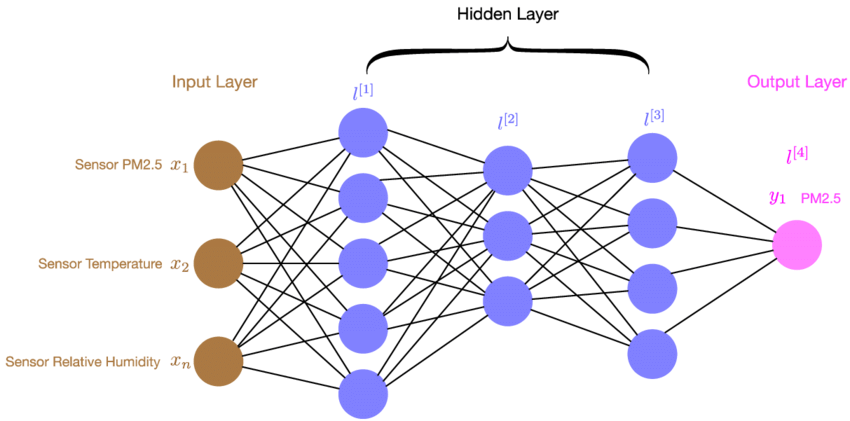
\includegraphics[scale=0.4]{pic/C3/c3_p2-2}
\caption{Adopting CWT for the Conversion of one-dimensional traffic data to two-dimensional scalogram.}
\label{fig:c3_p2-2}
\end{figure*}

\textbf{\subsubsection{Wavelet transform}}
Wavelet transform (WT) is a processing tool for extracting coefficients from a signal by using a wavelet function to turn it into wavelets [ 11]. WT decomposes data into coefficients and off er that information in sub scales. In this dissertation, we utilized continuous wavelet transform (CWT) for converting time series signal to time frequency images for detecting abnormalities in traffic patterns as depicted in Figure 2. {Equation \eqref{eq:2}} presents the mathematical expression for the CWT.

\begin{equation}
CWT_{x}^{\psi}= \frac{1}{\sqrt{|S|}} \int_{}^{}x(t) \psi^{*} (\frac{t-\tau}{S})dt 
\label{eq:2}
\end{equation}
where $\tau$ depicts the transition factor which is shift term to move the mother wavelet and $S$ denote the scale factor which is the frequency inverse. $x(t)$ represents the function of the mother wavelet. $\psi^{*} (\frac{t-\tau}{S})dt $ depicts the derived function from the mother wavelet. Low frequency corresponds to large S and small S leads to high frequency.


\textbf{\subsubsection{Convolution Neural Network}}

CNN is a sophisticated deep neural network based on visual perception that was first employed in the field of computer vision and has already shown great promise [12] 12]. CNN has recorded tremendous achievement in various applications especially detecting anomalies in radiographs [ 13]--[ 16]. With image as input, CNN may learn the hierarchical features to create a final set of high level
abstraction features, which are then sent to a fully connected layer as the classifier for categorical classification purposes. CNN learns the patterns in the images automatically and stores them in the network connection settings, requiring very little manual design. Furthermore, when compared to manual feature creation,
CNN is better at detecting intricate patterns in high dimensional data.




\textbf{\subsubsection{Proposed Wavelet Convolution Neural network}}

As shown in Figure 3 the proposed WavCovNet is a deep learning architecture that combines convolution layers in groups with wavelet decomposition layers generated from multi resolution analysis (MRA) f or DDoS attack detection . Two dimensional time frequency images with three channels are used as inputs to the proposed network. The resulting detail component from the first stage of decomposition is used as input to the first convolution
block, which is made up of two convolution layers.

After the approximate components of the first disintegration stage is further sub sampled to produce detail and approximate components of the second disintegration stage, the detail component of the first disintegration stage is fed as input to the second block, which comprises of two convolution network layers. It's worth mentioning that the detail component is concatenated through a channel of $1 \times 1$ convolution layer with a $64$ kernel size before being transferred to the second block to maintain a match in feature dimensionality with the output from the first block.

In the same fashion, the third and fourth blocks are treated same. At the third disintegration stage, the concatenation to the third block through the channel, on the other hand, is done via two $ 1 \times 1 $ convolution layers with kernel sizes of $64$  and $128$  respectively. The fourth block is made up of three convolution neural layers and average pooling, which is concatenated with the final decomposition level. Three $ 1 \times 1 $ convolution layers of $64$, $128$, and $256$ are used to achieve channel wise concatenation.



It's worth noting that the images are scaled down by a factor of two throughout the wavelet decomposition process. The fifth block is made up of two fully connected layers, and a classifier as the last fully connected layer with two class . We trained for $30$ epochs with a learning rate of $10^{4}$, $16$ as the batch size , and Adam as the optimizer. Training, validation, and test are the three sets of dataset split. During the training phase, the model's performance is also scrutinized. The suggested model is assessed using the test set split to obtain the final performance. Our model's performance was evaluated using well known metrics.

\textbf{\subsubsection{Experimental Detail and Setup}}

The core approach of the methodology is divided into two parts: data pre processing and feature extraction and learning. The raw DDoS data is transmitted to the network for the pre processing phase. Using digital signal processing met hods like CWT, the most significant and dependable underlying features are retrieved in the
pre processing step by converting the raw one dimensional traffic DDoS data to time frequency scalogram image data.


In this work, we trained our model for DDoS attack detection with continuous wavelet transform and wavelet convolutional neural network as a combined framework while using an Adam optimizer and dropout to avoid over fitting, early stop techniques is introduced and a learning rate of $10^{4}$ is used in order to obtain a better performance. We implemented the proposed model using Keras library with Tensorflow as back end on GeForce GTX 1080 GPU, which is driven by a parallel computing platform and programming paradigm called CUDA.

\textbf{\subsubsection{Performance Measures}}
We have applied some evaluation metrics in terms of accuracy, sensitivity, specificity and AUC on our proposed model. {Equation \eqref{eq:3}--\eqref{5}} are the numerical expression for the evaluation metrics.

\begin{equation}
Accuracy = \frac{TP+TN}{TP+TN+FP+FN}
\label{eq:3}
\end{equation}

\begin{equation}
Sensitivity = \frac{TP}{TP+FN}
\label{eq:4}
\end{equation}

\begin{equation}
Specificity = \frac{TN}{TN+FP}
\label{eq:5}
\end{equation}

\textbf{\subsection{Results and discussion}}
According to the automatic feature extraction method
depicted in {Figure \ref{fig:3}}, extensive experimental findings and discussion are presented in this section. The proposed attack detection system of DDoS is constructed on the Keras framework and utilizes Tensorflow as the back end. During the training and testing, we analyzed the proposed scheme for DDoS attack detection based on binary classification for both detecting and identifying incoming and outgoing DDoS attacks in smart grid networks. For detecting DDoS attacks, the proposed approach achieves 98.9\% accuracy.

\begin{table}[]
\caption{Performance comparison of our proposed model with selected pre-trained models.
WavCovNet model}
\label{tab5}
\begin{tabular}{lllll}
\toprule
\textbf{\multicolumn{1}{l}{Model}} & \textbf{\multicolumn{1}{l}{ACC (\%)}} & \textbf{\multicolumn{1}{l}{SEN (\%)}} & \textbf{\multicolumn{1}{l}{SPE (\%)}} & \textbf{\multicolumn{1}{l}{Time (Min)}} \\ \hline
\midrule
EfficientNet                & 95.1                         & 94.8                         & 95.2                         & 38                              \\
MobileNet V3                & 94.8                         & 95.4                         & 94.8                         & 41                              \\
DenseNet                    & 94.8                         & 95.7                         & 95.3                         & 51                              \\
ResNet 101                  & 94.6                         & 94.4                         & 95.8                         & 46                              \\\hline
\multicolumn{1}{l}{Ours}  & \multicolumn{1}{l}{98.9}    & \multicolumn{1}{l}{99.8}    & \multicolumn{1}{l}{99.9}    & \multicolumn{1}{l}{36}         \\ \hline
\bottomrule
\end{tabular}
\end{table}


{Figure \ref{fig:4}} depicts the training and validation accuracy curves of the proposed model which show that the model converges smoothly without over fitting. Figure 5 shows the gradual and steady reduction of the training and validation loss curves the proposed model. Generally, the performance of the proposed wavelet convolutional neural network is satisfactory. It is important to examine the validity of the proposed model in terms of the receiver operating characteristic curve (ROC) which shows the overall accuracy of the proposed scheme in terms of area under curve (AUC).


Figure 6 shows that the proposed model has high sensitivity associated with high specificity which minimizes the rate of false positive and maximizes the rate of true positive. Our proposed model achieves 99.8\% sensitivity and 99.9\% specificity as presented in Table 1. Table 1 shows the outcomes of our proposed methodology versus some pre-trained scheme. It is evident that the proposed technique outperformed the selected pre-trained methods by 3.8\% when it came to recognizing DDoS attack patterns in terms of accuracy. In addition, when compared to the pre-trained techniques, the proposed method obtained 3.2\% increase in sensitivity and a 3.1\% increase in specificity. ResNet-101 recorded the least score in accuracy (94.6\%) and sensitivity (94.4\%) whereas MobileNet-V3 recorded the least score in specificity (94.8\%). The proposed scheme is computational efficient with the least training time of 36 minutes as depicted in Table 1. Though DenseNet performed slightly better than ResNet-101, MobileNet-V3, and EfficientNet in accuracy, sensitivity, and specificity respectively but recorded the highest training time of 51 minutes for 30 epochs.

\textbf{\subsection{Conclusions}}

According to recent cyber-attack statistics, distributed denial of service (DDoS) attacks is the most common in smart grid infrastructure, and they are increasing in frequency and intensity over time. CNN models have acquired a lot of traction in image categorization applications as a result of their superior performance. However, CNN models are built to discover patterns in images therefore; they do not function as expected when trained on one-dimensional traffic data. In this paper, we proposed a method for converting a one-dimensional traffic data into two-dimensional time-frequency domain images in order to take advantage of CNN's potential. Following that, we trained our proposed WavCovNet on the converted data and evaluated its performance in recognizing DDoS attacks. The proposed approach detected DDoS attacks with 99.9\% accuracy, which is 9\% better than the pre-trained models. 


\end{document}
        % Chapter 3 contents inside the chapter folder
\documentclass{standalone}
% preamble: usepackage, etc.
  
\begin{document}
\chapter{Wavelet Convolutional Capsule Network}
\label{Chapter4}
Image identification, classification, natural language processing, object detection, and segmentation, are the few problems that modern machine vision applications need answers to. Due to the inability of traditional machine learning to solve these complicated issue due to its strict coding constraints, deep learning approaches such as convolutional and recurrent neural networks have been introduced. It is important to mention that classical CNN models are data hungry and are unable to recognize object pose and location details, thereby prompting the development of capsule networks. 

%%%%%%%%%%%%%%%%%%%%%%%%%%%%%%%%%%%%%%%%%%%%%%%%%%%%%%%%%%%%%%%%%%%%%%%%%%%%%%%% Paper 2 %%%%%%%%%%%%%%%%%%%%%%%%%%%%%%%%%%%%%%%%%%%%%%%%%%%%%%%%%%%%%%%%%%%%%%%%%%%%%%%%%%%%%%%%%%%%%%%%

\textbf{\section{Shared Weighted Continuous Wavelet Capsule Network for Electrocardiogram Biometric Identification}} 

Despite various usability and security issues, conventional passwords remain the most used method of internet authentication [1]-[3]. Passwords are inconvenient for users since they must be remembered and preferably, be lengthy and distinct. As a result, it should come as no surprise that many users choose weak passwords that they reuse across several platforms [4], [5], resulting in account hack and personal data breaches. According to studies, over 50\% of users use the same authentication credentials for several platforms [4] and over 80\% of privacy breaches are caused by poor authentication credential behavior [6]. 

Alternative authentication techniques, such as push notifications [7], graphical passcodes [8], and trust scores [9], and gestures [10], have been investigated in attempt to replace or supplement standard passwords. Biometric authentication is of particular importance due to its unique characteristics of user identity. Biometrics enhances usability of the system by eliminating the need for users to remember passwords or move about with a token at all times. The simplicity with which biometrics can be used for authentication has sped up their adoption in both the private and public sectors, with the global market for biometric technology anticipated to hit \$59.31 billion by 2025 [11].

While much of the previous research has focused on standard biometrics like fingerprints, facial recognition, and iris scans, there has been little work done to investigate new biometrics. In this paper, we look at a biometric based on electrocardiogram (ECG) signals, which represent the electrical activity of the human heart. ECG has been shown to be adequately unique to every person in previous studies [12] and could be utilized for identity verification. In this paper, we proposed a hybrid scheme of continuous wavelet transform (CWT) and capsule network for biometric authentication based on ECG.CNN has made significant progress in a variety of applications, particularly in detecting anomalies in radiographs [13] – [16]. 

%\begin{figure*}[t!]
%\centering
%\includegraphics[scale=0.1]{C4/c4_p2-1}
%\caption{Proposed scheme for detecting DDoS attack on smart grid.}
%\label{fig:c4_p2-1}
%\end{figure*}

While biometrics are more usable than standard passwords, there are still issues about biometric data security and privacy [17]. Biometrics cannot be readily reversed once they have been infiltrated, as they are based on an individual's lasting physiological or behavioral features. Additionally, biometric recognition system operators may gain undesired information from a user's biometric data. Fingerprint patterns, for example, may be linked to certain disorders [18]. In conclusion, some biometric traits, such as a person's face, are difficult to conceal. As a result, even if a person wants to remain unknown, they may be recognized without their consent or knowledge [18].

The heart is a muscular organ that supplies blood to the body's tissues via blood vessels [19]. The heart muscle must contract in order to supply blood, resulting in an electrical impulse. During an electrocardiogram (ECG) examination, this impulse can be measured on the surface of the body using electrodes put on the skin. The process of depolarization and repolarization of the heart chambers, which causes them to contract and rest, is captured by an ECG tracing.


Various researchers have looked into the ECG's peculiarity and stability. The majority of these are based on a "on-the-person" approach "a method for signal acquisition in which electrodes are placed directly on the person [20]. There are limited researches that use "off-the-person" methodology "They use a different approach, but they show a real-life application scenario for ECG identification systems. Placing ECG sensors into a smartphone cover, wristbands, and car steering wheel are just a few instances. Additionally, as shown in [20], previous researches frequently employ data acquired from a single data acquisition session which are easy to develop. 

In this work, CWT is utilized to convert the 1-dimensional time-series signal of ECG to 2-dimensional time-frequency scalogram as input image of distinct features with growing sensitivity which makes it suitable for CNN model to extract feature for training. The image features obtained from CWT are utilized to train the proposed capsule network for biometric authentication. We adopted some well-known evaluation metrics to validate the performance of the proposed scheme. 
Conclusively, we assess the effectiveness of the proposed scheme using public dataset and also presented some comparison with other methods of biometric authentication.

\textbf{\subsection{Methodology}} 
The proposed method for biometric identification using ECG is described in this section. Figure 1 depicts the general framework of the proposed scheme for user identification. First, the dataset utilized in this study for ECG biometric identification is properly described. 

\textbf{\subsubsection{Dataset}} 

Instead of creating a new dataset, we used an already existed dataset. For this study, we used the MIT-BIH Normal Sinus Rhythm available on Physionet database. The Physionet MIT-BIH Normal Sinus Rhythm database consists of healthy ECG records of persons between the ages of 20 and 50 with no major arrhythmias collected at the Arrhythmia laboratory of Boston’s Beth Israel Hospital[21]. Compared to other ECG dataset, Physionet MIT-BIH dataset has been utilized by most studies. Physionet MIT-BIH dataset consists of 30 recordings of normal sinus rhythm signals.


\textbf{\subsubsection{Proposed siamese capsule network (WavCapNet)}} 

This research proposes a siamese capsule network, as shown in Figure 3. The model accepts two scalogram images as inputs, and then transmits them into a shared weighted framework. The obtained data is forwarded into the fully-connected layer, and the model then determines if the outcome is valid or invalid. Our proposed model's method is based on a real-world security assessment of person identity.

In a real-world scenario, tenants of a specific building or employees of a company with access control security equipment are normally asked to go through a security check. These persons' biometric templates must have been stored in the system. When a person attempts to enter an authorized building or organization, a comparison of both the template and the query input is performed to determine whether the request is valid or invalid. As a result, the idea of employing a siamese capsule network to receive both ECG trait images, access their attributes, and determine whether they are similar or not is proposed. In general, a siamese network is used to compare two input images with similar weights and parameters. The extracted feature vectors of the two inputs are then obtained from the last layer, and the Euclidean distance is computed. If the distance between the two images is large, they are different, otherwise, they are similar.

\begin{figure*}[t!]
\centering
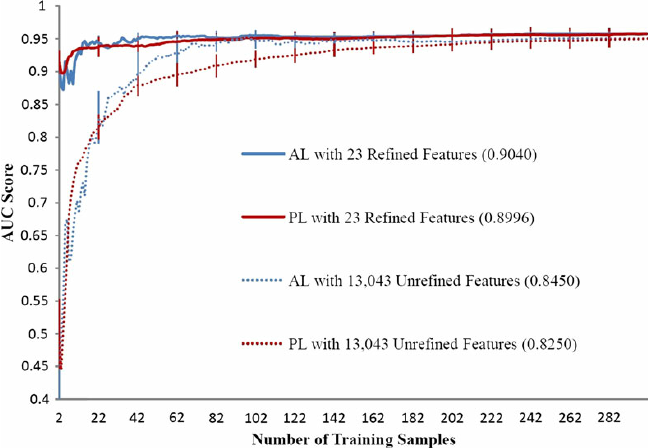
\includegraphics[scale=0.4]{C4/c4_p2-4}
\caption{Training and validation accuracy curves showing the performance of our proposed.}
\label{fig:c4_p2-4}
\end{figure*}

Computing the similarity of the ECG images will be omitted in our investigation, and instead the relationship between the two images will be utilized to predict the outcome. As a result, the distance calculating aspect of our work is eliminated, as shown in Figure 3. For feature extraction, a shared weighted capsule network with modified AlexNet as the base neural network is used, then the retrieved features are fused and passed into the fully-connected layer, and ultimately, the ECG images are predicted using a sigmoid classifier. Instead of the usual max-pooling layer, we introduced discrete wavelet pooling to replace the first and second max-pooling layers for down-sampling operation whereas the third max-pooling layer is eliminated to arrive at a feature vector of $256 \times 14 \times 14 $. The likelihood of which ECG trait matches the query or not is represented by the prediction result which is either 0 or 1.

\textbf{\subsubsection{Experimental detail and setup}} 

The basic technique of the proposed scheme is split into two phases: data pre-processing and feature extraction. The pre-processing step begins with the collection of raw ECG signals from the Physionet database. The most essential and consistent fundamental characteristics are obtained in the pre-processing step by converting one-dimensional time domain ECG signal to time-frequency domain image of two-dimension using CWT. This work employed continuous wavelet transform and siamese wavelet capsule networks trained on Physionet MIT-BIH ECG dataset for biometric identification using Adam optimizer and dropout to prevent over-fitting, early stop strategies, and a learning rate of $10^{4}$ to improve performance. Keras library with Tensorflow as the backend on a GeForce GTX 1080 GPU is used for the implementation of this work. Accuracy, sensitivity, specificity and AUC are some of the evaluation metrics applied on our proposed model. 

\begin{table}[]
\caption{Performance comparison of our proposed model with selected pre-trained models.
WavCovNet model.}
\begin{tabular}{lllll}
\toprule
\multicolumn{1}{l}{Model} & \multicolumn{1}{l}{ACC (\%)} & \multicolumn{1}{l}{SEN (\%)} & \multicolumn{1}{l}{SPE (\%)} & \multicolumn{1}{l}{Time (Min)} \\ \hline
\midrule
ResNet-101                  & 95.7                         & 95.8                         & 94.6                         & 47                              \\
EfficientNet                & 94.7                         & 94.3                         & 95.8                         & 40                              \\
MobileNet-V3                & 95.2                         & 94.5                         & 95.9                         & 39                              \\
DenseNet                    & 96.6                         & 95.4                         & 96.3                         & 46                              \\ 
\multicolumn{1}{l}{Ours}  & \multicolumn{1}{l}{99.2}    & \multicolumn{1}{l}{98.6}    & \multicolumn{1}{l}{99.5}    & \multicolumn{1}{l}{48}         \\ \hline
\bottomrule
\end{tabular}
\label{tab6}
\end{table}


\textbf{\subsubsection{Results and discussion}} 
The proposed ECG biometric identification scheme is built using the Keras framework and Tensorflow as the backend. We examined the proposed strategy for ECG biometric identification based on binary classification for both query match and mismatch in security access control systems during training and validation. The proposed approach obtains 99.2\% accuracy rate for identifying query match and mismatch. The proposed model's training and validation accuracy curves are depicted in Figure 4, which show that the model converges smoothly without over-fitting. The proposed scheme's training and validation loss curves are gradually and steadily reduced as shown in Figure 5. In general, the proposed siamese wavelet capsule network's performance is reasonable. It's crucial to evaluate the proposed model's validity using the receiver operating characteristic curve (ROC), which depicts the proposed scheme's overall accuracy in terms of area under the curve (AUC). Figure 6 illustrates that the proposed scheme has a high sensitivity combined with a high specificity, resulting in a low false positive rate and a high true positive rate.


As shown in Table 1, our proposed approach obtains 98.6\% sensitivity and 99.5\% specificity. The results of our proposed scheme versus certain pre-trained models are shown in Table 1. When it comes to correctly determining query match and mismatch of ECG characteristics, the proposed strategy clearly outweighed the selected pre-trained techniques by 2.6\% in terms of accuracy. In addition, the proposed method achieved 2.6\% increase in sensitivity and 3.2\% increase in specificity when compared to pre-trained procedures. EfficientNet had the lowest accuracy (94.7\%) and sensitivity (94.3\%) scores, whereas ResNet-101 had the lowest specificity score (94.6\%). It is worth noting that the proposed scheme has a slightly higher computational time of about 48 minutes in training but achieves the best result, as shown in Table 1. Though MobileNet-V3 had the shortest training time of 39 minutes, our proposed model still achieves satisfactory performance. 

\textbf{\subsubsection{Conclusions}} 

Biometric identification systems provide several benefits that traditional techniques do not. We proposed an ECG-based biometric identification system for security access control in this research, in which a continuous wavelet transform (CWT) was utilized to convert one-dimensional time-domain signals into scalograms of two-dimensional images to obtain good quality training data. A siamese capsule network framework was utilized to predict the right match or mismatch of ECG query samples using the extracted specific attributes from the scalograms. The findings show that the ECG signal is a reliable biometric measure that is resistant to noise and artifacts. Furthermore, the proposed security system's efficiency was assessed using both classification metrics and the ROC-AUC measure. The proposed scheme properly predicted ECG query samples with 99.2\% accuracy, which is 2.6\% higher than the other models.


%%%%%%%%%%%%%%%%%%%%%%%%%%%%%%%%%%%%%%%%%%%%%%%%%%%%%%%%%%%%%%%%%%%%%%%%%%%%%%%%%%%%%%%%%%%%%%%%%%%%%%
\end{document}        % Chapter 4 contents inside the chapter folder
\documentclass{standalone}
% preamble: usepackage, etc.
\begin{document}
\chapter{Conclusion}
\label{Chapter5}
Due to the obvious increased output of large amounts of information in recent times, particularly images, it is becoming necessary to build techniques and software for the automatic collection, processing, and analysis of such information in order to extract trends and patterns. This guarantees that images and its characteristics are converted by algorithm into representations that reflect their context and interpretation. Currently, innovations in artificial intelligence are being applied to system algorithms for image analysis and complicated analysis in the field of machine vision. Image classification and recognition are essential components of machine vision. 


\section{Research Findings}
In this dissertation, we examined the application of wavelet multi-resolution analysis and deep learning models as a single framework for the task of machine fault diagnosis, biometric identification and disease classification. 

\section{Contributions}
In this dissertation, we presented wavelet multi-resolution analysis algorithm and deep learning model as a single framework capable of attaining and advancing the horizon of research in medical imaging, machine fault diagnosis and biometric identification. 

In Chapter 2, We analyzed and presented the impact of existing approaches using both classic and cutting-edge techniques.

In Chapter 3, we developed an  image classification and identification for the feature extraction and classification of images.

In Chapter 4, we presented an improved capsule network for accurately classifying images. The images becomes the input data to the wavelet capsule network for feature extraction and classification.


\section{Future Works}
Given the vast amount of research in vision recognition and image classification, there are still a number of obstacles to overcome before reaching same accuracy of that of human. To begin, our models are supervised framework, which necessitates a large quantity of data to learn the mapping from an input $X$ to a label $Y$. 

As a result, achieving unsupervised artificial general intelligence appears to be a promising study area and natural next step in the advancement of machine intelligence in all areas.

\end{document}        % Chapter 5 contents inside the chapter folder
\include{chapter/c6}        % Chapter 6 contents inside the chapter folder
\include{chapter/c7}        % Chapter 7 contents inside the chapter folder

% the images and diagrams are organized in a separate folder called c1, c2, c3, .... and so on, inside the Pic folder

%\documentclass{standalone}
% preamble: usepackage, etc.
\begin{document}
	
前方高能,非战斗人员请撤离
弹幕  护体
弹幕  护体
弹幕  护体
弹幕  护体


\begin{landscape}
\begin{table}[t]
\caption{System corrections of the learning strategies for a relatively longer test sentence}
\label{table4}       % Give a unique label

\begin{tabular}{p{6cm} p{13cm}  } %{ll|l|l|l|l}

\hline
\hline
\textbf{System} & \textbf{Sentence}  \\
\noalign\hline
Source    
&But I disegree this opinion because often the advertisement do n't speak about the only functionals of the product but it promises other characteristics that do n't depend by it .   \\

\hline\hline
Two-tier seq2seq \(\Theta_{B_0}\leftarrow\Theta_{B_1}\), \(S^*\)                     
&But I \textcolor{red}{agree} this opinion because often the advertisement do n't speak about the only functionals of the product but it promises other characteristics that do n't depend by it .   \\

\hline
Three-tier seq2seq  \(\Theta_{B_0}\leftarrow\Theta_{B_1}\leftarrow \Theta_{B_2}\), \(S^*\)    
&But I \textcolor{blue}{disagree with} this opinion because often the advertisement do n't speak about the only functionals of the product but it promises other characteristics that do n't depend by it . \\

\hline
Two-tier seq2seq \(\Theta_{B_0}\leftarrow\Theta_{X}\), \(S^*\)      
&But I \textcolor{red}{agree} \textcolor{blue}{with} this opinion because often the advertisement do n't speak about the only functionals of the product but it promises other characteristics that do n't depend by it .\\

\hline
Three-tier seq2seq \(\Theta_{B_0}\leftarrow\Theta_{X}\leftarrow \Theta_{Y}\), \(S^*\)	     
&But I \textcolor{blue}{disagree with} this opinion because often the advertisement do n't speak about the only functionals of the product but it promises other characteristics that do n't depend by it .  \\

\hline\hline

Two-tier seq2seq \(\Theta_{B_0}\leftarrow\Theta_{B_1}\), \(S^{**}\)		               	        
&But I \textcolor{blue}{disagree with} this opinion because often the \textcolor{blue}{advertisements} do n't speak about the only \textcolor{blue}{functions} of the product but it promises other characteristics that do n't depend by it . \\

\hline
Three-tier seq2seq \(\Theta_{B_0}\leftarrow\Theta_{B_1}\leftarrow \Theta_{B_2}\), \(S^{***}\)		    
&But I \textcolor{blue}{disagree with} this opinion because often the \textcolor{blue}{advertisements} do n't speak about the only \textcolor{blue}{functions} of the product but it promises other characteristics that do n't depend \textcolor{blue}{on} it .   \\

\hline
Two-tier seq2seq  \(\Theta_{B_0}\leftarrow\Theta_{X}\), \(S^{**}\)			                     
&But I \textcolor{blue}{disagree with} this opinion because often the \textcolor{blue}{advertisements} do n't speak about the only \textcolor{blue}{functions} of the product but \textcolor{red}{it fails to express others .} \\

\hline
Three-tier seq2seq \(\Theta_{B_0}\leftarrow\Theta_{X}\leftarrow \Theta_{Y}\), 
\(S^{***}\)			
&But I \textcolor{blue}{disagree with} this opinion because often the \textcolor{blue}{advertisements} do n't speak about the only \textcolor{blue}{functions} of the product but \textcolor{red}{it fails to express others .} \\

\hline\hline
Reference 0	   &But I \textcolor{blue}{disagree with} this opinion because often the advertisement \textcolor{blue}{does n't} speak about only the \textcolor{blue}{functionality} of the product , but it promises other characteristics that do n't depend \textcolor{blue}{on} it .  \\

\hline
Reference 1	  &But I \textcolor{blue}{disagree with} this opinion because often the \textcolor{blue}{advertisements} do n't speak about the only \textcolor{blue}{functions} of the product , but it promises other characteristics that they do n't deliver \textcolor{blue}{on} .  \\

\hline
Reference 2	  &But I \textcolor{blue}{disagree with} this opinion because often the advertisement \textcolor{blue}{does n't} speak about the \textcolor{blue}{function} of the product but it promises other characteristics that do n't depend \textcolor{blue}{on} it .  \\

\hline
Reference 3	  &But I \textcolor{blue}{disagree with} this opinion because often the advertisement \textcolor{blue}{does n't} just speak about the \textcolor{blue}{functionality} of the product but it promises other characteristics that do n't depend on it .  \\
\noalign{\smallskip}\hline\hline\noalign{\smallskip}

\multicolumn{2}{l}{Note: }\\
\multicolumn{2}{l}{{\(S^*\) - The model was trained with the NUCLE dataset.}}\\
\multicolumn{2}{l}{{\(S^{**}\) - The model was trained with the NUCLE and FCE datasets }}\\
\multicolumn{2}{l}{{\(S^{***}\) - The model was trained with NUCLE, FCE
and Lang-8 datasets.}}
\end{tabular}
\end{table}
\end{landscape}

\end{document} %若需添加第六章请用这个模板修改

% misc
\documentclass{standalone}
% preamble: usepackage, etc.
\begin{document}

\thesisacknowledgement
First and foremost, I want to express my gratitude to my supervisor, Professor Jian Ping Li, who transformed me into a successful researcher through his patience, advice, and rigorous tutoring. Your prompt suggestions and counsel guided me in the right route, allowing me to achieve my PhD ambitions. I appreciate your confidence in me and the pleasant relationship you established with me during my academic years. I have learned a great deal from you, not only in terms of academics, but also in terms of overall development.

My research partner, Grace Ugochi Nneji, has been a huge source of inspiration for me over the last few years. Your regular motivation, interactions, and remarks influenced the direction of my studies and pushed me to achieve more. Your contributions were important elements of my foundation. It has also been a great pleasure to work with my Wavelet Analysis and Active Media Technology and Big Data Research Lab colleagues. Your suggestions and participation have helped to make my journey memorable and productive.

In addition, I owe a debt of appreciation to certain friends who have had a significant impact on my life. This includes Ariyo Oluwasanmi, Folarin Mordecai Raji, and Akeem Shokanbi. Your wishes, support, and care created an environment that was positive and conducive to my mental and physical health. Thank you for being such a wonderful people.

Thank you to UESTC's International Student Education Office and the entire School of Computer Science and Engineering. Finally, I would like to offer my heartfelt appreciation to my family for their unwavering support. During the difficult moments, I find consolation in your love and wishes. I owe everything I am to my late mother who was always willing to help me become the man of my dream.


\end{document}  %致谢
\thesisloadbibliography[nocite]{reference}  %参考文献


% comment while no need
%\documentclass{standalone}
% preamble: usepackage, etc.
\begin{document}

\thesisappendix

\end{document}   %附录,论文若无附录则用%将该命令取消
\thesisloadachievement{publications}  %攻读学位期间取得的成果,若无成果则用%将该命令取消
%\documentclass{standalone}
% preamble: usepackage, etc.
\begin{document}

\thesistranslationoriginal
\section{A Tight Upper Bound on Bit Error Rate}

\end{document}  %外文资料原文,论文若未引用外文资料则用%将该命令取消
%\documentclass{standalone}
% preamble: usepackage, etc.
\begin{document}

\thesistranslationchinese
\section{基于多载波索引键控的正交频分多路复用系统模型}

\end{document}   %外文资料译文,论文若未引用外文资料则用%将该命令取消

\end{document}
